%!TEX root = base.tex

\chapter{Experimental Methodology}

This chapter begins by presenting the overall rationale for the experimental
approach used to evaluate the theoretical model. Subsequent sections will
describe a particular experiment.

During the course of this master thesis project the primary challenge of
analysing performance of Felemban-Ekici models was accurate capture of network
performance statistics. In total, three different experiments were designed,
evaluated and executed. From the onset only one experiment was thought to be
needed, something that rather quickly was proven wrong. Each experiment lead
to a deeper understanding of the network system and how various systems affect
the results.

To provide a better foundation for analysing the results presented in Chapter
5, this chapter will, in addition to an overview, also try to provide some of
the knowledge needed to grasp the characteristics of each experiment.
Discussion of experiments and their results will be presented in the final
chapter.

Finally, this chapter will describe the experimental evaluation of the model
with real-world statistics.

\section{Overview}

As mentioned in the introduction, in order to solve the primary problem it has
to be partitioned into more manageable pieces. The problem discussed in this
section is ``\emph{Problem 3} - how should the definition of \emph{usefulness}
be evaluated?''.

The premise is as follows: in order to evaluate a theoretical model there must
first exist some set of data provided by the model itself, and an equivalent
set of data to compare against.

In this report, the data provided by the model are referred to as the
\emph{model metrics}. The other dataset, the comparison set, is gathered from
a specific device and referred to as the \emph{captured metrics}.

The general methodology of the model evaluation consists of iteration between
selection of model metrics and captured metrics until both datasets can be
compared.

Thus the answer appears to be: \emph{Construct an experiment and collect
metrics that have either a direct or indirect counterpart in the theoretical
model. If these metrics match numerically the theoretical model is useful. If
these metrics don't match numerically the theoretical model can still be
considered useful if the trends of these metrics match. If not, the model is
not useful.}

So the methodology essentially is designing experiments based on knowledge of
a device and its system, to obtain a set of \emph{captured metrics} that can
be compared with a similar set of \emph{model metrics}.

\section{Model Metrics}

As stated earlier, in order to know what to capture we must first select relevant
metrics from the model. A first step is to list some model parameters:

\begin{itemize}
	\item \emph{N} -- the number of network nodes
	\item $CW_{min}$ and $CW_{max}$ -- contention window min and max size
	\item \emph{E[D]} -- the mean payload size
	\item channel bit rate
	\item $L$ -- the \texttt{ShortRetryLimit}
	\item RTS/CTS -- the model presents models with basic access, RTS/CTS and a
	hybrid access scheme using a payload threshold
\end{itemize}

There are, of course, other parameters in the model, and certainly many more
parameters in the implementations of IEEE 802.11 (e.g. power saving, distance,
line-of-sight). These are, for the sake of tractability and real-world
usefulness, ignored and may contribute to significant errors. Our
argumentation is that any theoretical model must make decisions on what to
include in its scope, and any omissions are to be considered errors by model
divergence rather than circumstantial errors by environment. I.e. any error
thought to be due to variance outside model scope should be considered error
due to model design.

As described earlier, the Felemban-Ekici model provides normalized throughput
($U$), channel access delay and conditional packet collision probability.

Normalized throughput is constructed upon the conditional packet collision
probabilities, payload distribution and a variant of channel access delay.

Thus the to most important \emph{model metrics} are \emph{conditional packet
collision probability} (i.e. the probability that a packet collides during
transmission) and \emph{channel access delay}, defined as ``the time from the
packet becoming the head of the queue until the acknowledgment frame is
received.''.

\emph{Conditional packet collision probability} is not an easy metric to
obtain since it is a very low-level metric.

The \emph{channel access delay} can be obtained by measuring the total time
described in Figure \ref{fig:timings}. Such a solution would require radio
equipment not available for this thesis. A key insight is that, in a
controlled experiment, most of the parameters in Figure \ref{fig:timings}
actually are constant. The only dynamic parameter is the time spent in
backoff, $T_{\text{BACKOFF}}$.

With a set of \emph{model metrics}, it now becomes a game of trying to exploit
the device to obtain a set of comparable \emph{captured metrics}.

% TODO: flytta till diskussion
% However, after implementing the model, severe differences regarding the
% normalized throughput were discovered. While the re-implementation achieves
% packet collision probabilities similar to the original paper, no realistic
% tuning of throughput calculation parameters could reproduce the original
% values found in the paper. Thus this value is not generated by the
% re-implemented model, but rather compared to the curves found in the paper.

\section{Experiment 1: Wireshark}

% 	\item jana + wireshark pcap time capture (naive) -- A first attempt at
% 	capturing network timing statistics using Wireshark (libpcap).

The first experiment designed used the industry-standard Wireshark program to
capture outgoing packet information. Built on libpcap, Wireshark uses a Linux
kernel feature called "packet taps" to "capture" packets. A timestamp for each
packet capture is recorded, along with other packet data, in a pcap logfile.

Naively, the corresponding \emph{channel access delay} was thought to be
obtainable to comparing the timestamps between a send program's call to
\texttt{sendto} and the ``capture time'' reported by Wireshark. This would, in
fact, be comparable to the complete timeline from Figure \ref{fig:timings}. No
\emph{captured metric} comparable to \emph{conditional packet collision
probability} could be constructed, simply due to the fact that Wireshark is
too high-level to know about IEEE 802.11 frame transmission failures.

The experiment was designed thusly:

\begin{enumerate}
	\item one server running a \texttt{jana} server (`jana -s 1 -t 60`)
	\item one client running a \texttt{jana} client in saturation mode (`jana -c <server> -t 60`)
	\item <client> logs timestamp before and after calling `sendto`
	\item wireshark (or `tshark`) running on client, captures outgoing packets to <server>
\end{enumerate}

By combining the timestamps ``before-sendto'' and ``packet-capture'', we,
by-definition have obtained the time it took to transmit this packet.

However, this design has a deep flaw which is not apparent without deeper
insight into the networking stack. As explained earlier, the ``packet tap''
feature from which Wireshark obtains packets is actually triggered when the
packet exits the kernel queueing system (qdisc) and handed over to the driver
for transmission. In addition, if the tap was triggered after packet
transmission this would, for throughput reasons, not be done per-packet and
thus include a significant error.

By placing the socket in ``non-blocking mode'', \texttt{jana} circumvents a
classic problem relating to the send buffert being full, resulting in a
blocking call until the kernel has freed up memory. A process that can take a
\emph{very} long time, relatively speaking.

Of course it took some time to realise that the data obtained from this design
was incorrect.

\section{Experiment 2: Queueing the Network System}

% \item jana + qdisc + sndbuf (hacker) -- A second attempt at capturing
% 	network timing statistics by modelling the Linux kernel's network system
% 	as a queuing system.

After a few weeks of research and thinking a new way of modelling the egress
path was found.


% \begin{itemize}



%



% 	\item TG799-vac: metrics quality -- The primary testing device provides
% 	network-related statistics via \texttt{ubus}. A first due dilligence smoke test
% 	was performed to reveal any significant issues with the reported data. I.e.
% 	"can we trust what we get?"

% 	\item TG799-vac rssi quality -- A special-case test for the reported RSSI
% 	(Relative Signal Strength Indicator) metric to find any obvious errors.

% 	\item Ekici-Felemban in the wild -- Map \emph{model metrics} to \emph{captured
% 	metrics} from a TG799-vac using \texttt{ubus}, and evaluate against dataset
% 	obtained from a production network.
% \end{itemize}

% The \emph{conditional packet collision probability} can be empirically obtained by
% finding the number of transmission collisons and transmission attempts:

% \[
% 	P(\text{collision}\|\text{transmission}) = \frac{tx_{collisions}}{tx_{success}+tx_{collisions}}
% \]

% Similarly, the \emph{model metric} \emph{channel access delay} can be obtained
% by measuring the total time described in Figure \ref{fig:timings}.


\section{Experiment 3: Hacking on the driver}

% 	\item jana + iwlwifi driver (smart) -- A third stab at capturing network
% 	timing statistics by modifying the \texttt{iwlwifi} Wi-Fi driver.

\section{Parameter Mapping}

As mentioned, experiments were performed using \texttt{jana} to set packet
rates and payload sizes, and \texttt{ubus} to interact with the router
firmware to retrieve data.

\section{Model Evaluation with Real-World Data}

The second round of model evaluation was based on data from end users. This
required tools for accessing the network interface statistics, matching a set of
\emph{router metrics} with the \emph{model parameters} and analysis of the
selected \emph{router metrics} to guard against bugs.

\subsection{Interface}

Network interface data can be accessed through various different interfaces. In
this thesis two programs were tried during exploratory testing, \texttt{ubus}
and \texttt{quantenna api}. In the end \texttt{ubus} was chosen due to its
broader range of statistics (both 2.4 and 5.0 GHz modems) and consistency of its
output (no corrupt/invalid JSON was found).

\subsection{ubus Metrics}
Selecting a set of metrics which are equivalent to the model parameters.

This required a good understanding oh how the constraints of the model affected
the selection of router metrics, e.g. the model separates CTS-RTS and Basic mode
while the router automatically decides which to use based on packet payload
size, which isn't available to any tool.

In order to evaluate the models we needed these metrics:

\begin{itemize}
\item rssi
\item nodes
\item logical tx/rx rates
\item physical tx/rx rates
\end{itemize}

\subsection{Metric analysis}

We must analyse the validity of the reported parameters.

Do this with experimentation in the radio lab.

We want to analyse the reported values for RSSI, SNR, broken \& valid IEEE
802.11 frames.

Using quantenna and wl API:s to query:
\begin{itemize}
    \item \texttt{ubus call wireless.radio.monitor get}
    \item \texttt{ubus call wireless.ssid.stats get}
    \item \texttt{ubus call wireless.radio.stats get}
\end{itemize}

\subsection{Traffic counters}

As noted above, one of the \emph{model parameters} is normalised throughput,
defined in \cite{felemban} as

\begin{equation}
U = \frac{P_{success}T_{payload}}{P_{success}T_{payload} + (P_{busy} -
P_{success})T_{collision} + (1 - P_{busy})T_{idle}}
\end{equation}

where $P_x$ is probability of $x$ and $T_y$ time of $y$, e.g. probability of successful transmission or time to send payload over channel.

There are no direct equivalent \emph{router metrics} available. Instead traffic counters such as $TX_{packets}$,
$RX_{packets}$, $TX_{bytes}$ and $RX_{bytes}$, are required to compute an average throughput, $N$

\begin{equation}
N = \frac{TX_{bytes} + RX_{bytes}}{t}
\end{equation}

\subsection{RSSI experiments}

Received Signal Strength Indicator (RSSI) is an important, and tricky, value. It
is important because it is often the only indicator of signal strength, and
tricky due to high variance between two chips, from same or different vendors,
suggesting that variance stems from a combination of hardware and software
factors \cite{lui}.

In order to establish whether the RSSI metric could be used or not, analysis had
to be done to verify the behavior, accuracy and variance of the reported values.
This was done in a shielded lab with low-to-no external interference and no self
interference from reflection.

Figure \ref{fig:rssi_setup} shows how the router, antenna and laptop were
set-up. Three experiment sessions were carried out to measure RSSI, about 5
minutes per session, with two different spectrum analysers.

The first test established the baseline rssi values when the system (laptop) was
idle, i.e. any network load originated from background services. The second test
was conducted using \texttt{iperf3} to push as much network load as possible,
see listings \ref{lst:router}, \ref{lst:client} and \ref{lst:rssi} for relevant
scripts. The third test was a control test with a different spectrum analyser,
but otherwise identical to the second test.

Scripts for parsing the spectrum analyser data and related heat map generator
are detailed in listings \ref{lst:mdrparse} and \ref{lst:mdrplot}.

The \emph{spectrum analyser data} was plotted as a heat map; frequency vs. time
vs. signal strength. This graph shows both how signal strength varies over time
and frequency. In contrast, the \emph{router metrics} only specify one RSSI
value and thus the resulting plot compares RSSI vs. time. The graphs can be
analysed individually for insight into system behavior and compared to see how
they relate.

\begin{figure}
\center
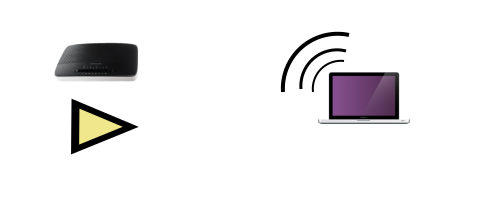
\includegraphics[width=0.9\textwidth]{images/rssi_setup.png}
\caption{TG799 router and measurement antenna side by side, 1 meter from laptop}
\label{fig:rssi_setup}
\end{figure}

\subsection{Evaluation}

Armed with a solid set of \emph{router metrics} data collection could begin.
Different scenarios were planned and tested.
